\documentclass[12pt]{report}
\usepackage{caption}
\captionsetup{font=footnotesize}
\usepackage{blindtext}
\usepackage{amsmath}
\usepackage{braket}
\usepackage{mathrsfs}
\usepackage{mathtools}
\usepackage{tikz}
\usepackage{graphicx}
\usepackage{caption}
\usepackage{subcaption}
\usepackage{subfig}
\usepackage[export]{adjustbox}
\usepackage{float}
\usepackage{csquotes}
\usepackage{esvect}
\usepackage{amsmath}
\usepackage[document]{ragged2e}
\usepackage{gensymb}
\usepackage{textcomp}

\usepackage{color}
\makeatletter
\patchcmd{\l@chapter}{1.0em}{0.5em}{}{}
\makeatother




\usepackage{geometry}
 \geometry{
 a4paper,
 bottom=40mm,
 left=30mm,
 top=30mm,
 right=26mm
 }

\renewcommand\bibname{References}

\begin{document}


  \begin{titlepage}
		\begin{center}
		    \vspace*{8ex}
			\hrule width \hsize \kern 1mm \hrule width \hsize
			\vspace{20pt} 
			\Large{\textbf{The Efficiency of Search Processes -- A Study using Phototactic Robotics }} %\\
			\vspace{20pt} 
			\hrule width \hsize \kern 1mm \hrule width \hsize
			 \vspace{25pt}
			{A Thesis submitted for}\\
			 the degree of  \\
			
			\vspace*{15pt}
			\large{\textbf{Bachelor of Science (Research)}}\\ 
			\vspace*{10pt}
			by\\
			\vspace*{15pt}
			\large{\textbf{Shadab Ahamed}}\\
			\begin{normalsize}
			Undergraduate Department\\
			Indian Institute of Science, Bangalore
			\end{normalsize}
			\vspace*{50pt}\\
		
				
			\begin{normalsize}
				{Under the guidance of}
			\end{normalsize}\\ 
			\large{\textbf{Dr. Manoj Varma}}
			\vspace*{2pt}\\
			\begin{normalsize}
				Robert Bosch Centre for Cyber-Physical Systems\\
					Indian Institute of Science, Bangalore
			\end{normalsize}
		\vspace*{5pt}\\
		April 2018
			\vspace*{5pt}\\
			{\includegraphics[scale=0.3]{IIsc_logo.jpg}}
		\end{center}
	\end{titlepage}


\newpage
\thispagestyle{empty}
\begin{center}

\end{center}
\newpage

\newpage
\thispagestyle{empty}
\begin{center}
\vspace*{\fill}
\textbf{ \textcopyright Shadab Ahamed\\ April 2018\\All rights reserved}
\vspace*{\fill}
\end{center}

\newpage
\thispagestyle{empty}
\begin{center}

\end{center}
\newpage


\newpage
\thispagestyle{empty}
\begin{center}
\vspace*{\fill}
DEDICATED TO\\
\vspace{25pt}
\textit{Indian Institute of Science, Bangalore}\\
\textit{where I spent four years of my life trying to do science.} 

\vspace*{\fill}
\end{center}
\newpage

\newpage
\thispagestyle{empty}
\begin{center}

\end{center}
\newpage


\thispagestyle{empty}
\section*{Certification}
\vspace{4ex}
\begin{justify}
The contents of the thesis titled ‘\textit {The Efficiency of Search Processes -- A Study using Phototactic Robotics}’ are based on the work done by Shadab Ahamed under the supervision
of Dr. Manoj Varma from August 2017 to April 2018 at the Robert Bosch Centre for Cyber-Physical Systems (RBCCPS), IISc towards the completion of his Bachelor of Science (Research) degree. This work is not a part of any previously submitted thesis. Appropriate
acknowledgments and citations have been provided wherever the work and contribution of others have been used.
\\

I hereby declare that I am the sole author of this thesis. I authorize Indian Institute of Science
to lend this thesis to other institutions or individuals for the purpose of scholarly research.
\end{justify}

\vspace{21ex}
\begin{minipage}{3in}
\textbf{Dr. S. Asokan} \\ {Instrumentation and Applied Physics}\\ {Indian Institute of Science}\\
{Bangalore-560012.}
\end{minipage}

\vspace{18ex}
\begin{minipage}{2.5in}
\textbf{Dr. Manoj Varma} \\ Robert Bosch Centre for Cyber-Physical Systems\\ {Indian Institute of Science}\\
{Bangalore-560012.}
\end{minipage}
\hfill
\begin{minipage}{2.5in}
\begin{flushright}
\textbf{Shadab Ahamed} \\ {Undergraduate Department} \\ {Indian Institute of Science}\\
{Bangalore-560012.}
\end{flushright}
\end{minipage}

\newpage
\thispagestyle{empty}
\begin{center}

\end{center}
\newpage


\pagenumbering{roman}
\addcontentsline{toc}{chapter}{\protect\numberline{} Acknowledgments}
\begin{justify}
\section*{Acknowledgments}
\vspace{4ex}
I would express my sincere gratitude to Dr. Manoj Varma,  for his infectious enthusiasm and the unyielding zeal with which he does science. He introduced me to the interdisciplinary field of Applied Complex Systems. It was a wonderful experience working with him. The frequent brainstorming sessions and the weekly group meetings proved to be critical for the successful completion of this project. I would also thank the Robert Bosch Centre for providing me with the state-of-art labs and other required facilities for carrying out my experiments. I would like to thank Mr. Muddu Krishna, who helped me with the intricacies of working with Arduino and the construction of phototactic robots. I would also thank my lab-members, especially  Divya Mohan, Avinash, and Navneet who made my stay in the lab enjoyable. 
Finally, I would thank KVPY for funding me throughout  my undergraduate years, and to
the Deans and Coordinators of the UG programme.


\newpage
\thispagestyle{empty}
\begin{center}

\end{center}
\newpage

\addcontentsline{toc}{chapter}{\protect\numberline{} Abstract}
\section*{Abstract}
\vspace{4ex}
Search and rescue robotics has become a hot topic of research in the past few decades. The challenges posed by this field of research include the procedures and algorithms used for searching the target and the subsequent administration of an efficiently implemented rescue plan. In this thesis, I have tried to focus on the former and summarized the theoretical basis of such movement and search processes which are essentially inspired from nature, i.e., organisms moving in their natural habitat for food and mates. Chapter 1 gives a brief introduction to the importance of movement and search by various organisms and tries to draw a parallel between these movement-search processes and reaction-diffusion process. Chapter 2 talks about normal and anomalous diffusion and defines an important quantity called the Hurst exponent. Chapter 3 argues for why a L\'evy procedure is beneficial for search tasks as opposed to Brownian motion and presents evidence from previous work. Chapter 4 briefly summarizes the experiments done using the phototactic robot and shows evidence for the higher efficiency of L\'evy searches. Finally, Chapter 5 lays down the concluding remarks and presents future scope for the work.    

\newpage
\thispagestyle{empty}
\begin{center}

\end{center}
\newpage

\addcontentsline{toc}{chapter}{\protect\numberline{} Contents}

\tableofcontents


\newpage
\thispagestyle{empty}
\begin{center}

\end{center}

\newpage
\pagenumbering{arabic}
\setcounter{page}{1}

\chapter{Movement and Search}

\section{Introduction}
Search processes are omnipresent in nature. The reactants involved in a biochemical process must find each other in order to convert into reaction products \cite{chemkin}. In the biophysical process, ligands search for binding sites \cite{bindsite}, proteins look for the target sequences on DNA \cite{DNA}. The animals must move in order to eat, mate and escape their predators, or even in search of suitable climate, temperature, nutrient concentrations, etc. The humans move from place to place in search of better education, shelter and livelihood.\\

The search for a specific target depends on a number of conditions and may take place in different environments. The targets may be sparse, hidden or difficult to detect even when found. They could be mobile or immobile, could try to evade the searchers \cite{evade, groupchase}, or be short-lived and might vanish even before getting detected. On the other hand, the searchers may be immobile too (as in the case of visual search \cite{visualsearch}), may move freely or interact with the environment. Their motion could be obstructed in the conditions of overcrowding \cite{overcrowding} (movement of proteins in the cell cytoplasm) or even facilitated in the presence of other entities (interaction with molecular motors). The searchers may search `blindly', detecting the target only upon a confrontation with it or can sense the target from long distances correcting their motion \cite{evade,chemotaxis}. They may not have the memory of the previously visited sites or may be adapted to avoiding already searched patches. Finally, the searchers may function individually or in a group/swarm \cite{chasing, unknownEnv}.\\


The problem of movement of organisms has been an important topic of research in the field of \textit{movement ecology} for many years. Given the ubiquity of moving organisms, a number of important questions arise naturally. For example, the priority in the order of driving factors that determine animal movement is not yet well understood and may even depend on the specific activity an organism is performing at a given time. However, there has been progress in understanding \textit{how} organisms move, i.e., what are the patterns of their trajectories. Figure \ref{fig:spdmk} shows the movement of spider monkeys in the Yucatan Peninsula when they were allowed to roam freely. What factors determine the shape and the statistical properties of such trajectories? Why do organisms move the way they do? What advantage do they gain from such a behavior? Moreover, how did the specific biological mechanism involved in generating the behavior evolve? \\
\begin{figure}[H]
\centering
\includegraphics[height=7cm, width = 7cm, keepaspectratio]{spider_monkey.png}
\caption{Movement patterns of spider monkeys in the Yucatan Peninsula, studied by Ramos-Fernández et al.\cite{spdmonkey} . Patterns generated by moving animals share features with random walks studied by physicists.}
\label{fig:spdmk}
\end{figure}

Similarly, the question of efficient search strategy has motivated a great deal of work in the last few years. The strategy employed by a searcher for efficiently detecting a target may be different in different situations, depending upon the searcher itself, the target and the surrounding. While earlier works have focussed on deterministic search algorithms \cite{deterministicAlgo}, such as those employed by humans in search of natural resources or rescue operations, more recent studies have argued in favor of random search strategies. It has been noted that in many cases, the strategies based on L\'evy flights or walks \cite{wanderingAlbatross, foraging}, in which a searcher performs excursions whose lengths are random variables with heavy-tailed distributions are more efficient than the conventional Brownian motion.\\

These types of questions are so closely connected to the areas such as random walk theory, stochastic processes and anomalous diffusion that they have attracted the attention of physicists \cite{optimalsearch}\nocite{levylikedetermine, masterEquation}--\cite{kineticsStochastics}.

\section{Biological encounters as a reaction-diffusion process}

Biological encounters generally involve a diffusive (transport) component and a reactive (interaction) component, such as eating or mating. Thus, they represent a special case of reaction-diffusion processes. The diffusion process is linear and the superposition principle holds for the probability density functions of the random walkers. On the other hand, the reaction process involves a particle interacting with another leading to nonlinear phenomena. For instance, consider the case of a predator wanting to eat its prey. In such a situation, we may consider two meals of the prey to be approximately twice as beneficial as a single meal, but $10^3$ meals are not approximately $10^3$ times as beneficial. As a result, the reaction between the predator and the prey deviates from the linear behavior.\\

The diffusion that accompanies such diverse reactions remains the same, at least in a first approximation. Specifically, we do not expect the randomness observed in the movements to depend strongly on whether the organism is foraging for food or searching for a mate or something else, so long as such relevant search cues as the density of organisms remain comparable. This assumption, to the extent that it remains approximately valid, justifies the study of diffusive properties of such encounter processes independently of the nature of the reactive processes. In this thesis, we will focus on the diffusive aspects of the underlying reaction-diffusion phenomena. 

\chapter{Random Walks}
\section{Central Limit Theorems}
The Gaussian curve occurs in nature ubiquitously due to the wide applicability of the central limit theorem, which states that the sum of a large number of statistically independent and identically distributed random variables that have finite variance converges to a Gaussian or a `bell-curve'.\\

For a long time, it was taken for granted that the sum of independent and identically distributed random variables always converges to a Gaussian distribution. It was later found out by Paul L\'evy, a French mathematician, that the Gaussian distribution is a special case of the more general L\'evy stable distribution.\\

Consider a sum $S$ of $N$ independent and identically distributed random variables. The probability density function of $S$ is equal to the Fourier convolution of the $N$ individual probability density functions for the $N$ random variables. The characteristic function is defined as the Fourier transform of the probability distribution function. The desired functional form for the L\'evy stable distribution probability density function must remain invariant under repeated convolutions with the probability density functions of the individual random variables. One can show that the most general stable characteristic function has a stretched exponential function form, from whose Fourier transform one can obtain the expression of the L\'evy stable distribution. The most general case, known as the skew L\'evy $\alpha$-stable distribution, is given by 
\begin{equation}
\phi(t) = \exp[it \nu - |ct|^\alpha (1 - i\beta sign(t)\Phi) ]
\end{equation}
\begin{equation}
\Phi = 
\begin{cases}
\tan(\alpha \pi/2), & \alpha \neq 1\\
-\frac{2}{\pi} ln|t|, & \alpha = 1
\end{cases}
\end{equation}
\begin{equation}
P(S) = \frac{1}{2 \pi} \int_{-\infty}^{\infty} dt \exp[-itS]\phi(t) 
\end{equation}
where $\nu$ represents a shift, $\beta$ is the asymmetry (hence the skewness) and $c$ is a scale. The L\'evy index $\alpha \in (0, 2]$ is the key parameter in the study of L\'evy flights and L\'evy walks. For $\alpha \in (0, 2)$, the probability density function has an asymptotic power-law tail with exponent $\mu = \alpha + 1$. It leads to closed-form expressions only in three special cases: Gaussian distribution ($\alpha = 2$) with variance $\sigma^2 = 2c^2$ and mean $\mu$, the Cauchy distribution ($\alpha = 1$, $\beta = 0$), and the L\'evy distribution ($\alpha = 1/2$, $\beta = -1$).

\section{Normal diffusion and Brownian motion}
The diffusion governed by Gaussian probability density function whose variance grows linearly in time is known as \textit{normal diffusion}. In this section, I briefly mention the two formalisms for treating normal diffusion based on the Langevin and Fokker-Planck equations\\

The Langevin equation is a stochastic differential equation for the velocity in terms of noise, typically a Wiener process. The numerical integration of Langevin equation gives to the trajectory of the walker.\\

We often have no information about the individual trajectories of the particles but only the probability density function for the walker's position. Hence, by considering an ensemble of non-interacting random walkers, the Langevin equation leads to a Fokker-Planck equation for the probability density function of a walker's position. The equation of the free random walkers subject to Wiener noise is given by the following case of Fokker-Planck equation (also known as the heat equation)
\begin{equation}
\frac{\partial}{\partial t} P = D \frac{\partial^2}{\partial x^2} P,
\end{equation}
where $D$ denotes the diffusion constant. For the initial condition of random walkers starting from the origin at time $t = 0$
\begin{equation}
P_0(x) = P(x, 0) = \delta(x),
\end{equation}
where $\delta(x)$ is the Dirac delta function, the solution is given by
\begin{equation}\label{eq:propagator}
P(x,t) = \mathcal{N}(t) \exp\Bigg[ -\frac{x^2}{4Dt}\Bigg],
\end{equation}
\begin{equation}
\mathcal{N}(t) = \frac{1}{\sqrt{4 \pi Dt}}
\end{equation}
Here, $P(x, t)$, the probability density function, is also known as the propagator because $P(x - x_0, t - t_0)dx$ is the probability of finding the random walker in the position interval $[x, x + dx]$ at time t if at an earlier time $t_0$, the walker's position was $x_0$. 
The propagator is of the form 
\begin{equation}
P(x, t) \sim \frac{F(x^2 /t)}{\sqrt{t}},
\end{equation} 
therefore,
\begin{equation}
\begin{split}
\langle x^2 \rangle &\sim   t\\
\langle x^{2n} \rangle &\sim t^n
\end{split}
\end{equation}
Hence, the moment grows in time according to 
\begin{equation}
\langle x^{2n} \rangle  \sim \langle x^2 \rangle^n
\end{equation}
As can be seen, the moments do not grow independently. Note that the quantity $\langle x^2 \rangle/t$ is constant. The constant of proportionality can be obtained from the equation \ref{eq:propagator}. The mean squared displacement thus grows as
\begin{equation}
\langle x^2 \rangle = 2Dt
\end{equation}

\section{Anomalous diffusion}
The phenomena of diffusion not described by normal diffusion in the long-time limit are known as \textit{anomalous diffusion} \cite{anomalousDiff}. A quantity known as the Hurst exponent $H$ is defined to quantify the variation of mean squared displacement with time $t$ \cite{hurst}, as $\langle x^2 \rangle \sim t^{2H}$. When the mean squared displacement grows superlinearly  in time ($H > 1/2$), it is known as \textit{superdiffusion} \cite{superSub}. When the scaling is sublinear ($H < 1/2$) in time, it is known as \textit{subdiffusion} \cite{superSub}. The main focus of this thesis is superdiffusion, with L\'evy flights and walks being the best examples.

\begin{figure}[H]
\centering
\includegraphics[height= 10cm, width = 10cm, keepaspectratio]{Hurst.png}
\caption{The uncorrelated Brownian motion has $H = 1/2$ due to the central limit theorem. The subdiffusive processes have $H < 1/2$. Localized and confined random walks have $H = 0$. The superdiffusive walks have $H > 1/2$ with $H = 1$, being the ballistic limit. The processes with $H > 1$ are known as superballistic motion which corresponds to accelerating particles. L\'evy flights and walks are superdiffusive \cite{physofforaging}.}
\label{fig:hurst}
\end{figure}



\subsection{Anomalous diffusion with H = 1/2}
Generally, the anomalous diffusion is defined as $H \neq 1/2$, but in a weaker sense, the anomalous diffusion can also include the $H = 1/2$ case, but with non-Gaussian probability density functions. For instance, the logarithm of stalk prices follows what seems to be a random walk, with $H = 1/2$ and the financial returns appearing uncorrelated. The absolute value of the random walk step-sizes possess long-range power-law correlations \cite{selfgenpowerlaw}. There are fat tails in the distribution of financial returns. The presence of long-range power-law correlations and fat tails in the probability density functions are inconsistent with the normal diffusion.

\subsection{Generalized Hurst exponents} 
Sometimes, the second moment (variance) is not sufficient to quantify the full behavior of the probability density functions. A thorough description sometimes may require an infinite number of moments. The generalized Hurst exponent $H(q)$ gives the scaling \cite{criticalscaling} of the other moments of the position of the random walker
\begin{equation}
\langle |x|^q \rangle \sim t ^{q H(q)}
\end{equation}
For Brownian motion and normal diffusion, $H(q) = H = 1/2$.\\

Monofractal walks have a single exponent $H(q) = H$, whereas multifractal walks have different (i.e. non-unique) $H(q)$ values for different $q$. The monofractal walks have a single scaling exponent (e.g. fractal dimension). Multifractal walks can be considered as consisting of many monofractal walks, each with its own scaling exponent. The probability density function for a multifractal walk starting at the origin changes its shape with time, whereas for the monofractal walk, it only widens while retaining the basic shape.\\

Note that monofractality does not imply normal diffusion. The fractional Brownian motion, described by the propagator 
\begin{equation}
P(x,t) = \mathcal{N}(t) \exp\Bigg[ -\frac{x^2}{4Dt^{2H}}\Bigg],
\end{equation}
\begin{equation}
\mathcal{N}(t) = \frac{1}{\sqrt{4 \pi Dt^{2H}}}, \quad \quad 0 < H < 1, \quad \quad H \neq 1/2
\end{equation}
is monofractal because $H(q) = H$. Yet, $H \neq 1/2$, so fractional Brownian motion does not produce normal diffusion. It is thus an example of monofractal anomalous diffusion that is caused by long-range power-law autocorrelations in the underlying noise that drives the random walk, thus disrupting the convergence to normal diffusion.\\

Another mechanism disrupting the convergence to normal diffusion in the long time limit is through the power-law tailed distribution in the random walk steps. For specific values of the power-law exponent, the random variables can have diverging variance, leading to L\'evy processes. The L\'evy flights (described in detail later) are monofractal. The propagator for the L\'evy walks has a much more complicated behavior but the long-time behavior becomes similar to that of the L\'evy flights \cite{levyFW, levyFW1}.

\subsection{Mathematical formalism for anomalous diffusion}

The most well-known approach for analyzing anomalous diffusion uses the formalism of continuous time random walks (CTRWs). CTRWs were first proposed by Montroll and Weiss \cite{CTRW, AsympSoltoCTRW}, and allow a generalization of the Wiener processes underlying Langevin equations. A more general distribution of the random walk \textit{jump sizes} and \textit{pausing times}  are introduced. \\

Consider a CTRW that allows a random walk step $j$ to take time $\tau_j$ and have a size $l_j$. The standard random walk corresponds to the special case $\tau = 1$ and $l = \pm 1$. One can expect the anomalous diffusion to arise via diverging moments for $l$ or $\tau$. Let $\psi(l, \tau)$ denote the joint probability density function for a step to have a length $l$ and take time $\tau$. The jump length and jump time probability density functions satisfy

\begin{equation}
\lambda(l) = \int_0^\infty  \psi (l, \tau)d\tau
\end{equation}
\begin{equation}
\omega(\tau) = \int_{-\infty}^\infty  \psi (l, \tau)dl
\end{equation}
The mean pausing time $T$ and the second moment of the jump size are thus given by
\begin{equation}
T = \int_0^\infty \tau \omega(\tau)d\tau
\end{equation}
\begin{equation}
\sigma^2 = \int_{-\infty}^\infty l^2 \lambda(l) dl
\end{equation}

A finite $T$ ensures that the number of jumps remains linear in $t$. Similarly, a finite value of $\sigma^2$ ensures that the central limit theorem holds. The anomalous behavior arises if either value diverges.

\chapter{L\'evy Flights and L\'evy Walks}

\section{Hurst exponents for L\'evy flights and walks}
The term \textit{L\'evy flight} was first coined by  Beno\^{i}t Mandelbrot. L\'evy flights and walks have found application in the study of various systems such as protein folding dynamics, cavity quantum electrodynamics, photonic superdiffusion, random lasers and materials through which photons execute a L\'evy walk, kinematics of ions in optical cavities, finance and economics, etc.\\

L\'evy flights arise when the jump size distribution has a power-law tail $\lambda(l) \sim l^{-\mu}$, leading to an infinite variance for $\mu < 3 $. The necessary and sufficient conditions of the central limit theorem do not hold in this case. The probability density function for the position of the walker converges to a L\'evy stable distribution with L\'evy index $\alpha = \mu - 1$, with $0 < \alpha \leq 2$. The special case of $\alpha = 2$ corresponds to normal diffusion.\\

When $\alpha < 2$, the system behaves superdiffusively,  with limit $\alpha \to 0$ being the ballistic case. As far as the diffusion is concerned, the tail of the propagator is of utmost importance. Note that for $\alpha < 2$, one cannot define the mean squared displacement because it diverges and as a result, one can only study moments of the order lower than $\alpha$. In this way, one can show that a pseudo mean squared displacement grows as $t^{1/\alpha}$ for L\'evy flights. A unique Hurst exponent characterizes the behavior of L\'evy flights
\begin{equation}
H = \frac{1}{\alpha} = \frac{1}{\mu - 1}
\end{equation}
The difference between L\'evy flights and L\'evy walks is interesting. L\'evy flight jumps take zero or negligibly small time, whereas a L\'evy walk proceeds at a constant velocity. A L\'evy flight is local in time, whereas a L\'evy walker takes $l_j/v$ units of time to move a distance of $l_j$ units due to finite velocity $v$. Hence, it is difficult to arrive at the scaling behavior of L\'evy walks. In order to understand their superdiffusive behavior, one can provide a non-rigorous but intuitive argument as follows: consider the case,  $\omega(\tau) \sim \tau^{-(1 + \alpha) }$, which is equivalent to taking $\lambda(l) \sim l^{-(1 + \alpha)}$ due to the space-time coupling
\begin{equation}
\begin{split}
t &\sim N, \quad \quad \quad 1 < \alpha < 2\\
x &= \sum_{i=1}^N l_i \\
\langle l^2 \rangle \sim& \int_0^t l^2  l^{-(1 + \alpha)} dl \sim t^{2 - \alpha}
\end{split}
\end{equation}

where $x$ denotes the position of the random walker expressed as the sum of individual steps $l_i$, $N$ denotes the number of steps taken until time $t$. $\langle l^2 \rangle$ is finite and growing in time, hence normal diffusion is possible but with a time-dependent diffusion constant. Specifically, $\langle x^2 \rangle$ should be proportional to $\langle l^2 \rangle$ because $\langle l^2 \rangle$ denotes the characteristic scale of the jumps
\begin{equation}
\langle x^2 \rangle \sim \langle l^2 \rangle t
\end{equation}
Substituting this value for $\langle l^2 \rangle$, we obtain the result
\begin{equation}
\langle x^2 \rangle \sim t^{3 - \alpha}, \quad \quad 1 < \alpha < 2
\end{equation}
Finally, we obtain the following long limit result for L\'evy walks.
\begin{equation}
H = \frac{3 - \alpha}{2} = \frac{4 - \mu}{2}, \quad\quad\quad 1 < \alpha < 2
\end{equation}
We thus observe that L\'evy walks have a scaling different from that of L\'evy flights. 

\section{L\'evy flight foraging hypothesis}
The L\'evy flight foraging hypothesis is stated as follows:
 \textit{since L\'evy flights and walks can optimize search efficiencies, therefore natural selection should have led to adaptations for L\'evy flight foraging} \cite{LFFH}.
The central concept uses the power-law distribution with exponent,   $\mu = \alpha + 1$ for the jump size distribution.
\begin{equation}
p(l) \sim l^{-\mu}, \quad \quad \quad l > l_0
\end{equation}
By changing the value of $\mu$, one can allow superdiffusive L\'evy searches as well as Brownian searches involving normal diffusion. The L\'evy index, $\alpha$ of the L\'evy flight propagator is for the range $1 < \mu \leq 3$, and $l_0$ is a lower cut-off where the power-law tail begins. The ballistic motions and normal diffusion described by Gaussian propagators represent the two extremes of L\'evy flights and walks regime. The ballistic motion corresponds to the limit $\alpha \to 0$, whereas $\alpha = 2$ is consistent with normal diffusion. L\'evy walks and flights correspond to the intermediate values of $\alpha$, a regime characterized by fat tails in the propagator and superdiffusive Hurst exponents $H > 1/2$.\\

\begin{figure}[H]
\centering
\includegraphics[height= 9cm, width = 9cm, keepaspectratio]{mu.png}
\caption{For steps of size $l$ drawn from a probability density function $P(l) = l^{-\mu}$, the resulting type of diffusion depends on the value of $\mu$. For $\mu > 3$, the central limit theorem guarantees convergence to normal diffusion. The ballistic limit corresponds to $\mu \to 1$. For $\mu \leq 1$, the distribution cannot be normalized. The intermediate values $1 < \mu < 3$ result in superdiffusive L\'evy flights \cite{physofforaging}.}
\label{fig:mu}
\end{figure}


The physics of foraging is nonintuitive and interesting in the cases where the target density is low (like scarcity of food). In such cases, the resource distribution doesn't seem to play an important role. For example, fish \cite{fish, fish1}, insects \cite{insect} and marsupials \cite{marsupial} have been shown to change their diffusiveness in scarce conditions by increasing movement actively, possibly as a neurophysiological response to the dearth of resources. This change in activity is in concordance with the idea of L\'evy flight foraging as a built-in evolutionary adaptation as opposed to an emergent property.

\section{Evidence for L\'evy foraging behavior}
Reynold \textit{et al.} studied butterflies \cite{butterfly} and have speculated that L\'evy flight searches might underlie visually prompted mate location in these organisms. In a separate study, they noted the behavior of \textit{Angrotis segetum} moths \cite{moth} and found complex flight patterns compatible with scale-free L\'evy flight searches.\\

The most convincing evidence of L\'evy walks includes a statistically rigorous study of bony fish, sharks, sea turtles and penguins by Humphries \textit{et al.}, published in 2010 \cite{marine}.\\

Forcadi \textit{et al.} \cite{deer} reported that fallow deer (\textit{Dama dama}) performs L\'evy walks while searching alone for food, with exponent $\mu = 2.16 \pm 0.13$. Though the L\'evy behavior could not be observed in clustered deer. Dai \textit{et al.} \cite{elephant} studied a herd of elephants in South Africa and showed that they follow a stochastic process known as the L\'evy-modulated correlated random walk.\\

A study by Bartumeus \textit{et al.} \cite{dinoflagellates} has investigated the flight times of dinoflagellate \textit{Oxyrrhis marina}. They found that the distribution of flight times switched from an exponential (diffusively equivalent to $\mu > 3, H = 1/2$) to an inverse square law distribution ($\mu = 2, H > 1/2$) when the prey (\textit{Rhodomonas}) decreased in abundance. In a separate research, Bartumeus also studied Mediterranean seabirds \cite{seabird} and found that when operating trawlers are present, their flight length distributions decay exponentially. On the other hand, when trawlers are absent, the seabirds appear to move superdiffusively. \\

\chapter{Experiments with the Phototactic Robot}
\section{Phototaxis}
The term \textit{phototaxis} is a portmanteau word with Ancient Greek origin, that literally translates to light (\textit{ph\^os}) + arrangement (\textit{taxis}). Phototaxis is characterized by the directional locomotory movement of organisms (or cells) in response to light \cite{phototaxis}. The movement may be either towards (\textit{positive phototaxis}) or away (\textit{negative phototaxis}) from the source of light. Organisms exhibiting positive phototaxis are \textit{Euglena} and photosynthetic bacteria. Certain insects like cockroaches exhibit negative phototaxis.\\


This chapter talks about the experimental setup of the phototactic robot, how the experiment was conducted and interpretation of results. In order to detect the spotlight (target) focussed at the centre of a square-shaped arena, the phototactic robot (searcher) was designed and programmed to implement a correlated random walk with (1) constant jump step sizes and (2) jump steps drawn from a power-law distribution $P(l) \sim l^{-\mu}$ with different values of $\mu$ in the range $1 < \mu \leq 3$. With this analysis, we have tried to show evidence in favor of the use of power-law distributed jump steps for maximizing the search efficiency. 

\section{The setup}
\begin{enumerate}
\item \textbf{Arena :} The arena (Figure \ref{fig:arena}) where the experiment was conducted is located at the Robert Bosch Centre for Cyber-Physical Systems, Indian Institute of Science, Bangalore. The dimensions of the square-shaped base of the arena are 3 ft x 3 ft (approximately, 90 cm x 90 cm). It consists of four opaque walls of height 1 ft ($\sim$ 30 cm) on the four sides  and a transparent glass ceiling/roof on the top.

\item \textbf{Torch :} The J Go SWAT Multifunction Rechargeable LED 50W Flashlight Torch with LUXEON 3 Watt LED Bulb was used for creating the spotlight at the centre of the arena. It was mounted at a height of 2ft 9in ($\sim $84cm) from the ceiling of the arena.

\begin{figure}[H]
\centering
\includegraphics[height=9cm, width = 9cm, keepaspectratio]{arena.jpg}
\caption{The arena where the experiments were performed. The illumination was done using an overhead torch (as seen in the figure above) and the robot was released from a point outside this illuminated region.}
\label{fig:arena}
\end{figure}


\item \textbf{Light-seeking \& obstacle-avoiding robot :} The robot (Figure \ref{fig:robot}) was built using the Arduino Uno platform, a microcontroller board based on the ATmega328 (datasheet). The chassis of the robot was build using cardboard and two DC motors were used to drive the two wheels (made from rubber). It consisted of two \textit{photosensors} to sense and detect light and an  \textit{ultrasonic sensor} to detect and turn back from the obstacles (in this case, the four walls of the arena). The entire robot was powered using a 3.7V, 2200 mAh Li-ion battery. All the programming was done in Arduino IDE.  

\begin{figure}[H]
\centering
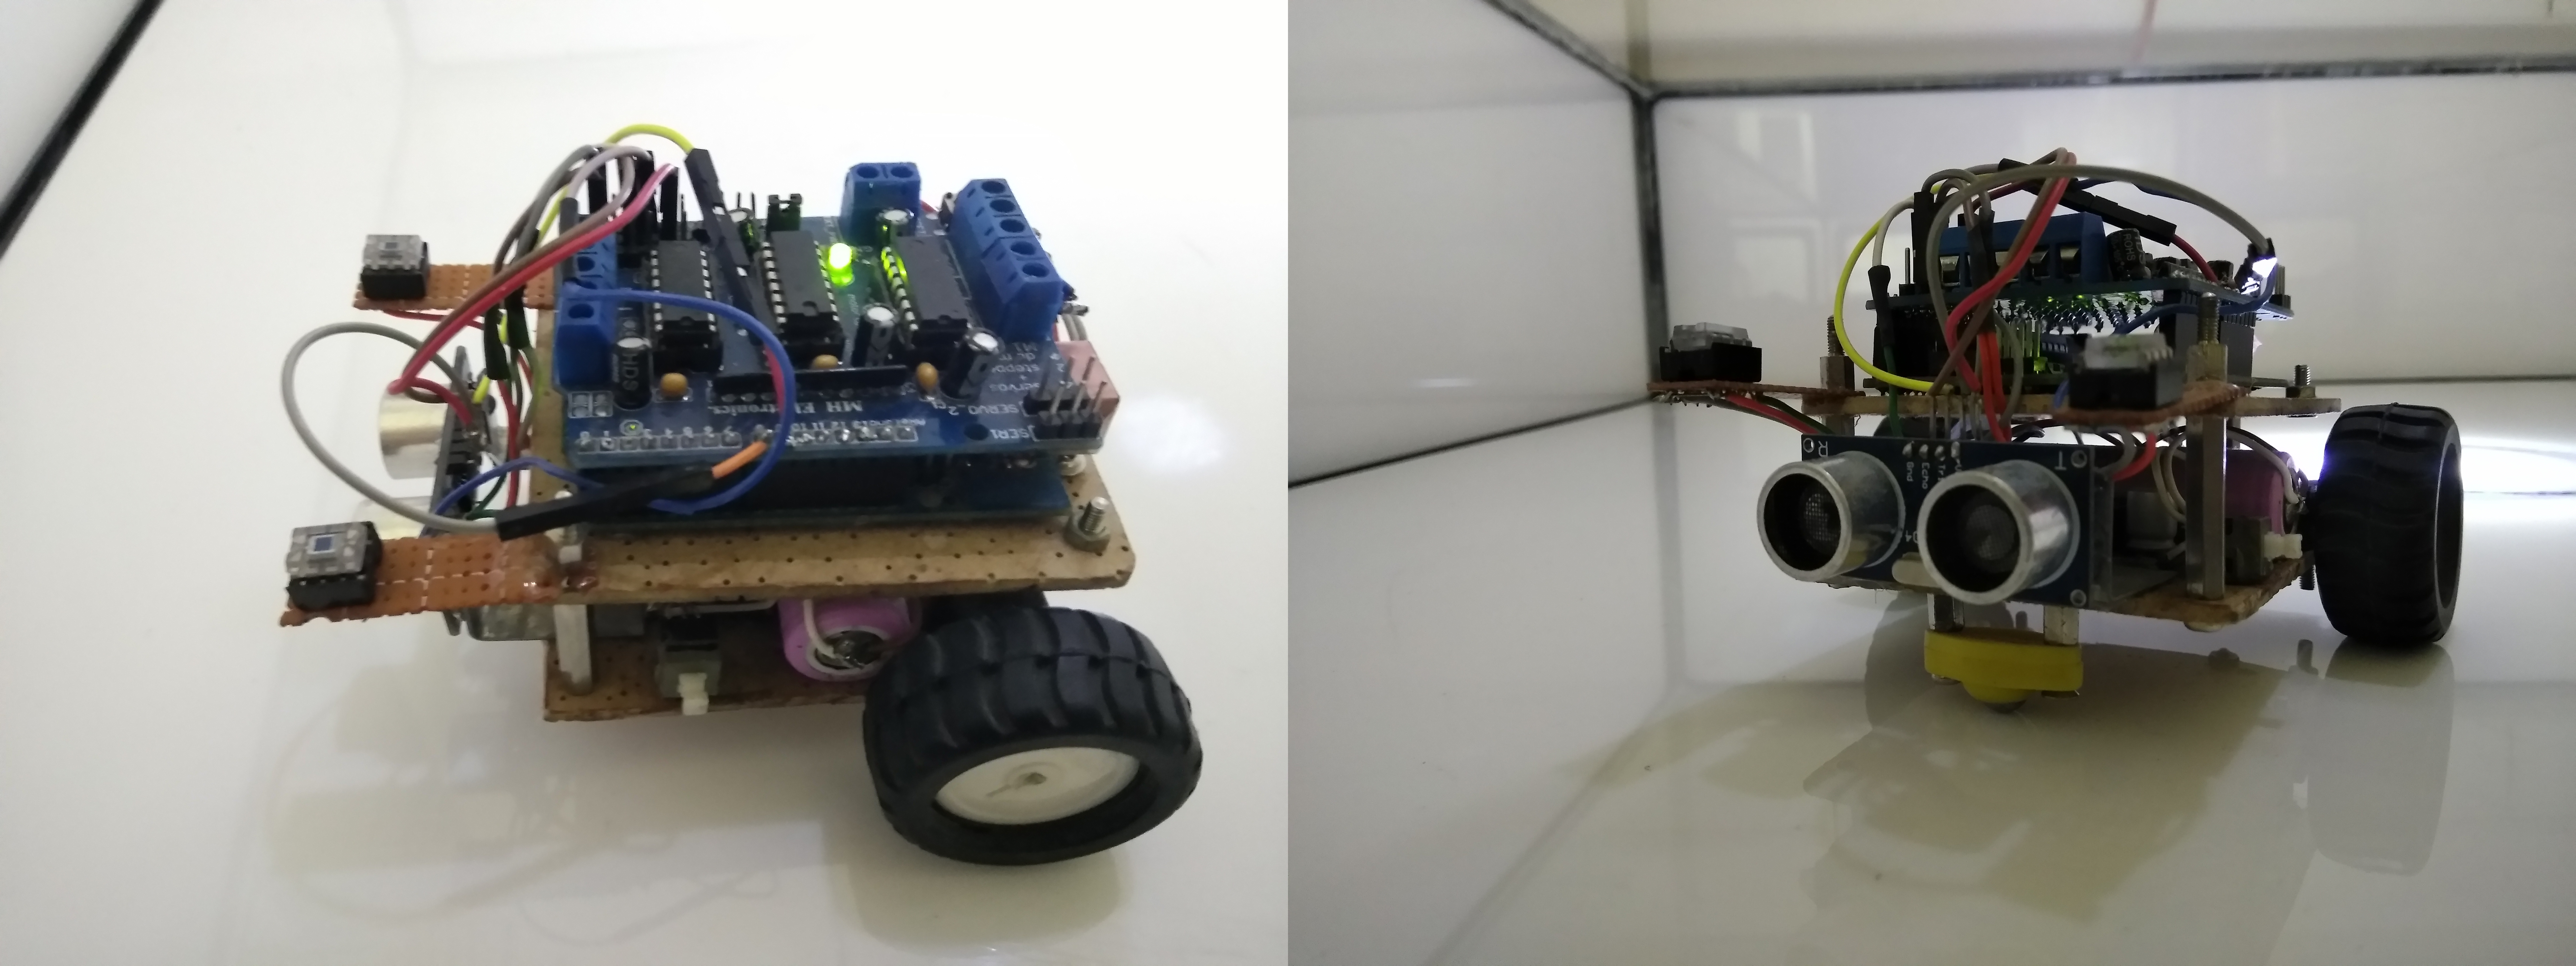
\includegraphics[height=12cm, width = 12cm, keepaspectratio]{robot_two.jpg}
\caption{Light-sensing \& obstacle-avoiding robot}
\label{fig:robot}
\end{figure}


\item \textbf{Photosensor :} Two OPT101 monolithic photodiodes and with on-chip trans-impedance amplifier were used as photosensors. The OPT101 operated from 2.7V to 36V supplies and quiescent current is only 120 $\mu$A.

\item \textbf{Ultrasonic sensor HC-SR04 :} This module emits an ultrasound of frequency 40000 Hz, which travels through the air and bounces back towards the module upon encountering an obstacle. The distance $d$ between the module and the obstacle is thus calculated using $d = v_0 t/2$, where  $v_0$ is the speed of sound in air (m/s) and $t$ is the time elapsed between the event when the sound was emitted and the reflected sound was detected. This module consists of 4 pins, \textit{Gnd}, \textit{Vcc}, \textit{Trig} and \textit{Echo}. The \textit{Gnd} and the \textit{Vcc} pins of the module was connected to the Ground and the 5 volts pins on the Arduino Uno Board respectively and the \textit{Trig} and \textit{Echo} pins to any Digital I/O pin on the Arduino Board. In order to generate an ultrasound, the \textit{Trig} pin was set on a HIGH state for 10 $\mu$s that sent out an 8 cycle sonic burst traveling at the speed of sound, and received at the \textit{Echo} pin after reflection from an obstacle. The \textit{Echo} pin then outputs the time (in $\mu$s) the sound wave traveled.





\item \textbf{DC motors :} Two GA12-N20 geared mini DC motors were used to drive the wheels, which had an RPM of 600 @ 6V, with a voltage rating of 6$\sim$12V.
\end{enumerate}

\begin{figure}[H]
\centering
\begin{subfigure}{.4\textwidth}
  \centering
  \includegraphics[height=5.2cm, width=5.2cm, keepaspectratio]{lightsensor.png}
  \caption{}
  \label{fig:sub1}
\end{subfigure}%
\begin{subfigure}{.4\textwidth}
  \centering
  \includegraphics[width= 4.5cm, height=4.5cm, keepaspectratio]{motor.png}
  \caption{}
  \label{fig:sub2}
\end{subfigure}
\begin{subfigure}{.4\textwidth}
  \centering
  \adjincludegraphics[height=4.5cm, width=4.5cm, keepaspectratio]{ultrasonic.jpg}
  \caption{}
  \label{fig:sub3}
\end{subfigure}%
\caption{(a) Block diagram of OPT101 monolithic photodiode, (b) GA12-N20 geared mini DC motor, (c) Ultrasonic sensor HC-SR04}
\label{fig:materials}
\end{figure}



\section{Experiments}

The diameter of the spotlight focussed at the centre of the arena was around 15 cm. The torch focussed the light beam only within this circular region and there was a sharp drop in the intensity outside this region. Hence, the outside area can essentially be treated as dark areas with no light (there was practically no light gradient upon moving outwards from the centre, even within the illuminated region). The length of sides of the arena was around 90 cm (roughly 6 times the size of the light spot). The robot was released from points lying on a circle of radius around 40 cm centered at the centre of the arena, with tangential orientation. The speed of the robot was fixed at 4 cm/s for the entire duration of the experiment. The motion of the robot was as follows: in the dark region, it moved forward for time $\Delta t$ (which could be fixed for subsequent forward motions or could be drawn from a probability distribution), then took a turn randomly by an angle  between 0-180\degree  as measured in the Cartesian coordinates. The previous two steps were repeated until the robot entered the light spot. Upon entering the light stop, the robot halts. Note that the turn angle was not uniformly distribution between 0-360\degree  and hence the motion is a correlated random walk, with the tendency to move in the forward direction with respect to the current orientation. Also, note that the robot doesn't sense light (or obstacles) while moving but only between the subsequent jump steps, and therefore it is possible for the robot to cross the light spot multiple times during the experiment and still not stop (because it entered the light spot while moving and not between the two jump steps).

\subsection{Constant $\Delta t$}  
The robot was programmed with constant forward jump times  $\Delta t = $ 1 s, 1.5s, 2s and 4s. The time taken to search the target, i.e. the \textit{search time} or \textit{time for convergence} was recorded. The experiment was repeated 60 times for each constant value of $\Delta t$. The \textit{cutoff time} was fixed at 10 mins (600s), i.e. the search time for a run that didn't converge within 10 mins was set to 10 mins. Figure \ref{fig:constT} shows the cumulative distribution function for the search time for various values of $\Delta t$. It can be seen that there is a transition between 2s and 4s, stating that given the experimental conditions,  the runs for $\Delta t < 2$s converge and for some value of $\Delta t > 2$s, the convergence is minimal. It can also be noted that for lower values of $\Delta t$, the convergence is more likely as well as efficient (more likely to take shorter time), as can be seen from the plot for 1s and 2s. There seems to be an anomaly as the efficiency for $\Delta t = $1.5s doesn't seem to lie between 1s and 2s, and it can be attributed to statistical errors which can be eliminated by taking more data.\\ 


\subsection{Power-law distributed $\Delta t$ }
This section gives an account of the experiments in which the jump time $\Delta t$ was drawn from a power-law distribution $P(\Delta t) \sim (\Delta t) ^{-\mu}$ with a heavy-tailed propagator. The values of $\mu$ were chosen such that $1 < \mu \leq 3$ to make the motion fall in the L\'evy flight regime. The values of $\Delta t$ in each case were drawn from the range [0.5s, 3s] based on the particular power-law distribution. From Figure \ref{fig:power}, it can be observed that a larger value of $\mu$ results in a more efficient search procedure. It is difficult to differentiate between the plots for $\mu = 2$ and $\mu = 1.5$ as they largely seem to overlap. An extra plot outside the L\'evy regime has been shown for $\mu = 4$ and it is evident that the efficiency dropped for the value of $\mu > 3$. This is because for $\mu > 3$, the second moments $\langle x^2 \rangle$ becomes finite and the motion resembles normal diffusion.  Hence, it can be safely concluded that larger the value of $\mu$ (within the L\'evy regime), the heavier is the tail, and more efficient is the search process. Also, for values of $\mu > 3$, the efficiency is likely to drop.

\begin{figure}[H]
\centering
\includegraphics[width = 14cm, keepaspectratio]{constant_T.pdf}
\caption{Cumulative distribution function for different constant $\Delta t$.}
\label{fig:constT}
\end{figure}

\begin{figure}[H]
\centering
\includegraphics[width = 14cm, keepaspectratio]{powerlawT_new1.pdf}
\caption{Cumulative distribution function for power-law distributed $\Delta t$ for different values of $\mu$.}
\label{fig:power}
\end{figure}




\chapter{Conclusion and Scope}
The aim of this thesis was to reiterate the importance of L\'evy searches in various systems. Section 3.3 presented the evidence for L\'evy foraging found in the animal kingdom. Similarly, the experimental work verified the claim that in a system with low target density, the L\'evy flight turns out to be more efficient than the correlated Brownian motion in the case of robotic random search.\\

Although a phototactic robot was used in the experiment, it would certainly be an interesting venture to have a similar search performed by a chemotactic robot looking for a chemical source such as ethanol, CO$_2$, etc. In the case of phototactic robotics, the target was localized and immobile. Chemotactic robotics will pose further challenges because the chemicals such as ethanol or CO$_2$ can quickly diffuse into the air and can have different concentrations in different areas, with an higher concentration near the chemical source and lower as one moves away from the source. It would rather be a harder problem to solve both in terms of the theoretical framework of L\'evy flight and designing and programming the robots to be able to efficiently perform the search in the case where the target is non-localized and fluctuating in the real time. Despite the difficulties, the problem will be quite compelling in the sense that the robot will be able to sense the target at a distance and the subsequent motion can be corrected accordingly. The concept of adaptive-L\'evy flights \cite{adaptLevy} can be used to design such systems. \\

Chemotactic robotics finds tremendous application in search and rescue operations. In times of natural calamities such as earthquakes, chemotactic robots fitted with CO$_2$ detectors can be efficiently used to detect the presence of humans stuck in places and whether they are still breathing. However, in such a scenario, the flexibility of the robots to be able to travel through small areas and bend around obstacles will play a bigger role in the rescue operation. Similarly, drones fitted with similar sensors can help deliver food packets in places where people are stuck due to an earthquake. \\

Another application of chemotactic robotics could be in the chemical industries involved in producing toxic gases such as CO as byproducts. Many robots moving on land and drones in air fitted with the respective chemical sensors can be collectively employed to perform the search task to detect and precisely pinpoint the location of leakage points. Such technological advancements will not only help prevent casualties in such industries but will also give rise to better robots with improved search abilities.\\

The L\'evy flight mechanism can be found even at the level of molecules and enzymes. When any situation presents many similar pairs of keys and locks, considerable time and energy are required to find the matching pairs. As the number of pairs grows, so does the time needed to find the right key-lock combinations. When a substrate approaches an enzyme, it can only bind to the active site of the enzyme to form an enzyme-substrate complex. The search halts only when the appropriate coupling takes place. Lomholt \textit{et al.} \cite{DNALevy} studied models of searches by proteins with targets on the DNA, combining normal diffusion and L\'evy type diffusion.\\

A lot has been studied and analyzed in the field of animal flight foraging but a lot more is still left to be studied and understood. Some important problems in the field are \cite{physofforaging}:
\begin{enumerate}
\item To what extent and under what circumstances do organisms move superdiffusively?,
\item Is such superdiffusive movement an adaptation or an emergent property?
\item What is the globally optimum search strategy for locating scarce, random, and
uniformly distributed targets?
\end{enumerate}
Though the ecologists are close to fully answering the first question, the other two still remain open, which would require newer investigations and future work.


\addcontentsline{toc}{chapter}{\protect\numberline{} References}

 
\bibliography{thesis}
\bibliographystyle{unsrt}
\end{justify}

\end{document}